\chapter{Theoretical Analysis}

\section{Circuit 1: Non-Inverting Amplifier}

\begin{figure}[h]
    \centering
    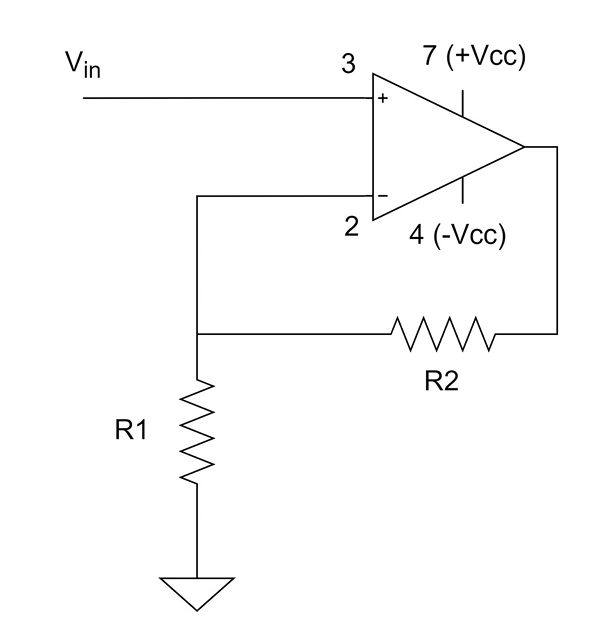
\includegraphics[width=0.5\textwidth]{assets/non-inverting.png}
    \caption{Non-Inverting Amplifier}
    \label{fig:non-inverting-amplifier}
\end{figure}

The non-inverting amplifier is a type of operational amplifier circuit that uses positive feedback to provide a closed-loop gain. The circuit is shown in Figure \ref{fig:non-inverting-amplifier}. The gain of the non-inverting amplifier is given by the formula:

\begin{equation}
    A = 1 + \frac{R_2}{R_1}
\end{equation}

In our case, $f = 1kHz$, $V_{in} = 100mV$, $R_1 = 1k\Omega$ and $R_2 = 22k\Omega$. Therefore, the gain of the non-inverting amplifier is:

\begin{equation}
    A = 1 + \frac{22k\Omega}{1k\Omega} = 23
\end{equation}

\noindent And expected output is calculated as:

\begin{equation}
    V_{out} = A \cdot V_{in} = 23 \cdot 100mV = 2.3V
\end{equation}

\newpage
\thispagestyle{plain}

\section{Circuit 2: Inverting Amplifier}

\begin{figure}[h]
    \centering
    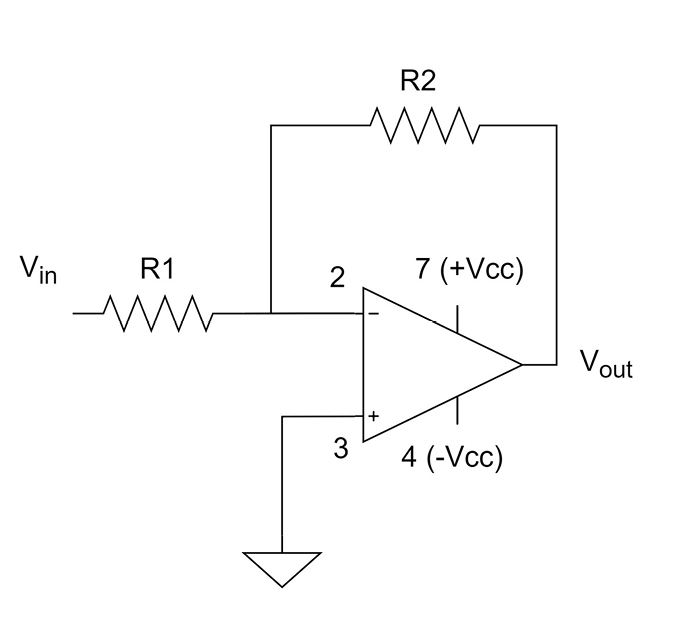
\includegraphics[width=0.5\textwidth]{assets/inverting.png}
    \caption{Inverting Amplifier}
    \label{fig:inverting-amplifier}
\end{figure}

Every calculation is similar to the non-inverting amplifier, except the gain formula. The gain of the inverting amplifier is:

\begin{equation}
    A = -\frac{R_2}{R_1}
\end{equation}

In our case, $f = 1kHz$, $V_{in} = 100mV$, $R_1 = 1k\Omega$ and $R_2 = 22k\Omega$. Therefore, the gain of the inverting amplifier is:

\begin{equation}
    A = -\frac{22k\Omega}{1k\Omega} = -22
\end{equation}

\noindent And expected output is calculated as:

\begin{equation}
    V_{out} = A \cdot V_{in} = -22 \cdot 100mV = -2.2V
\end{equation}

\newpage
\thispagestyle{plain}

\section{LTspice Simulation}

\subsection{Non-Inverting Amplifier}

\begin{figure}[h]
    \centering
    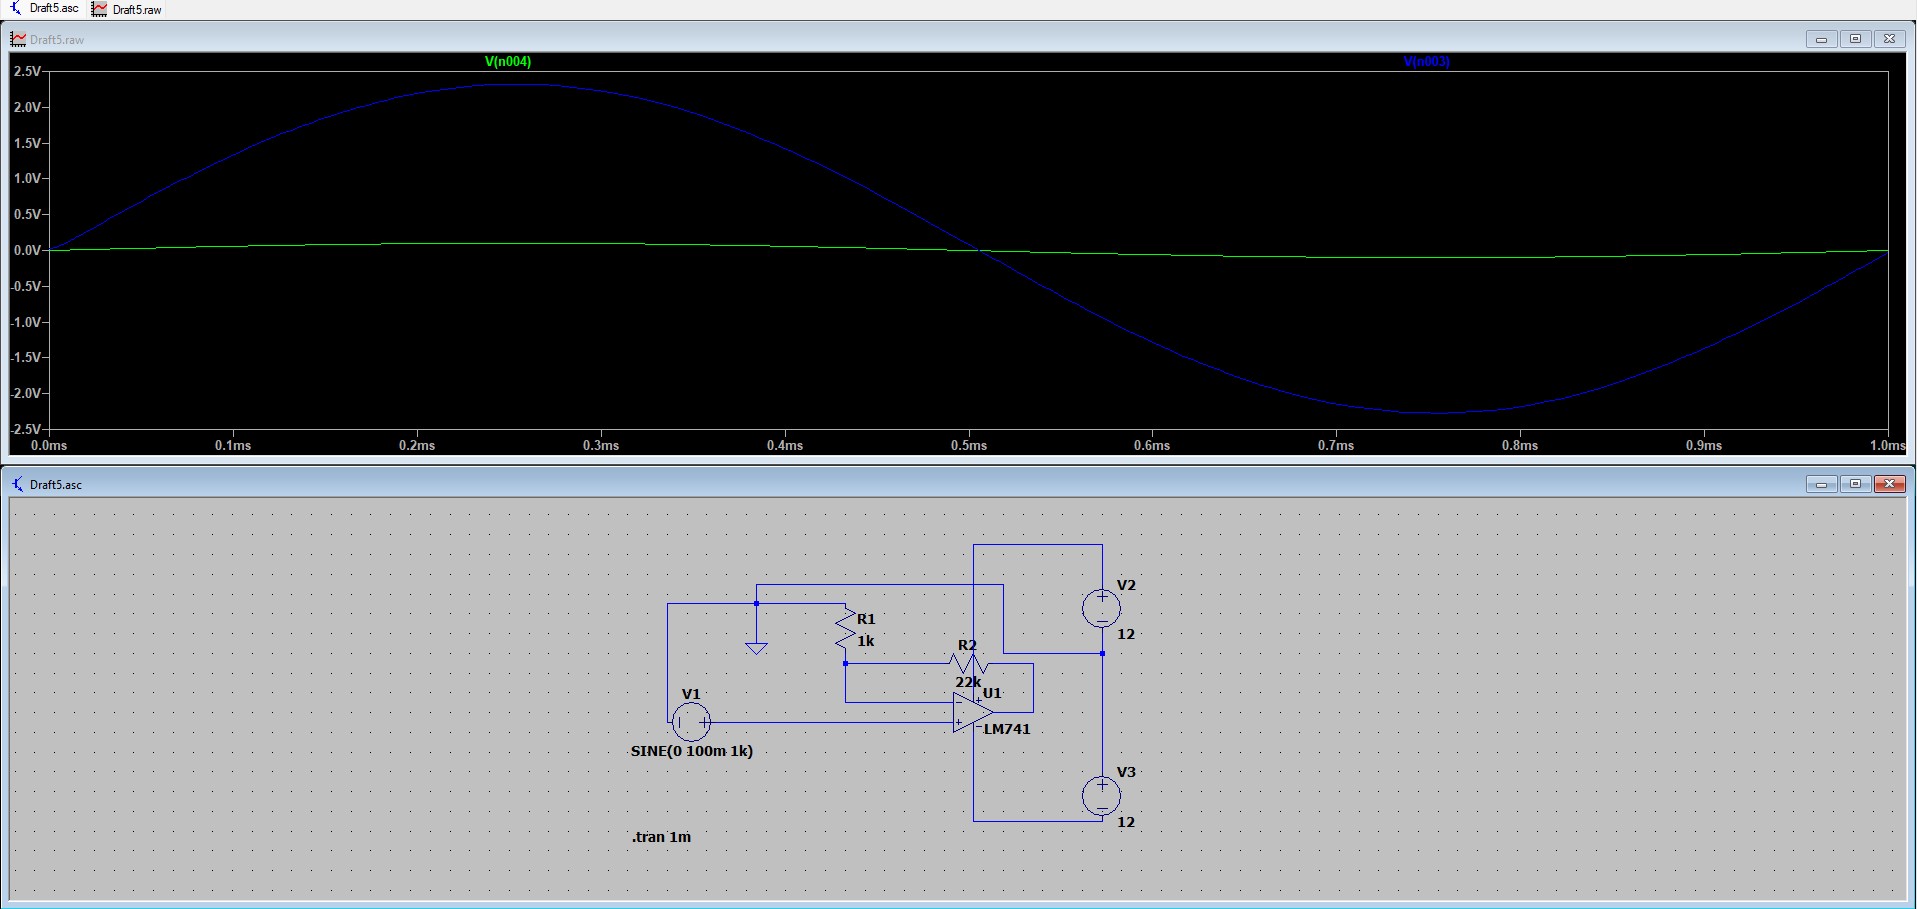
\includegraphics[width=1\textwidth]{assets/100m-non-inverting.png}
    \caption{Non-Inverting Amplifier @ 100mV}
    \label{fig:100m-non-inverting}
\end{figure}

Applying 100mV input to the non-inverting amplifier, the output is 2.3V as expected. The simulation result is shown in Figure \ref{fig:100m-non-inverting}. 

\begin{figure}[h]
    \centering
    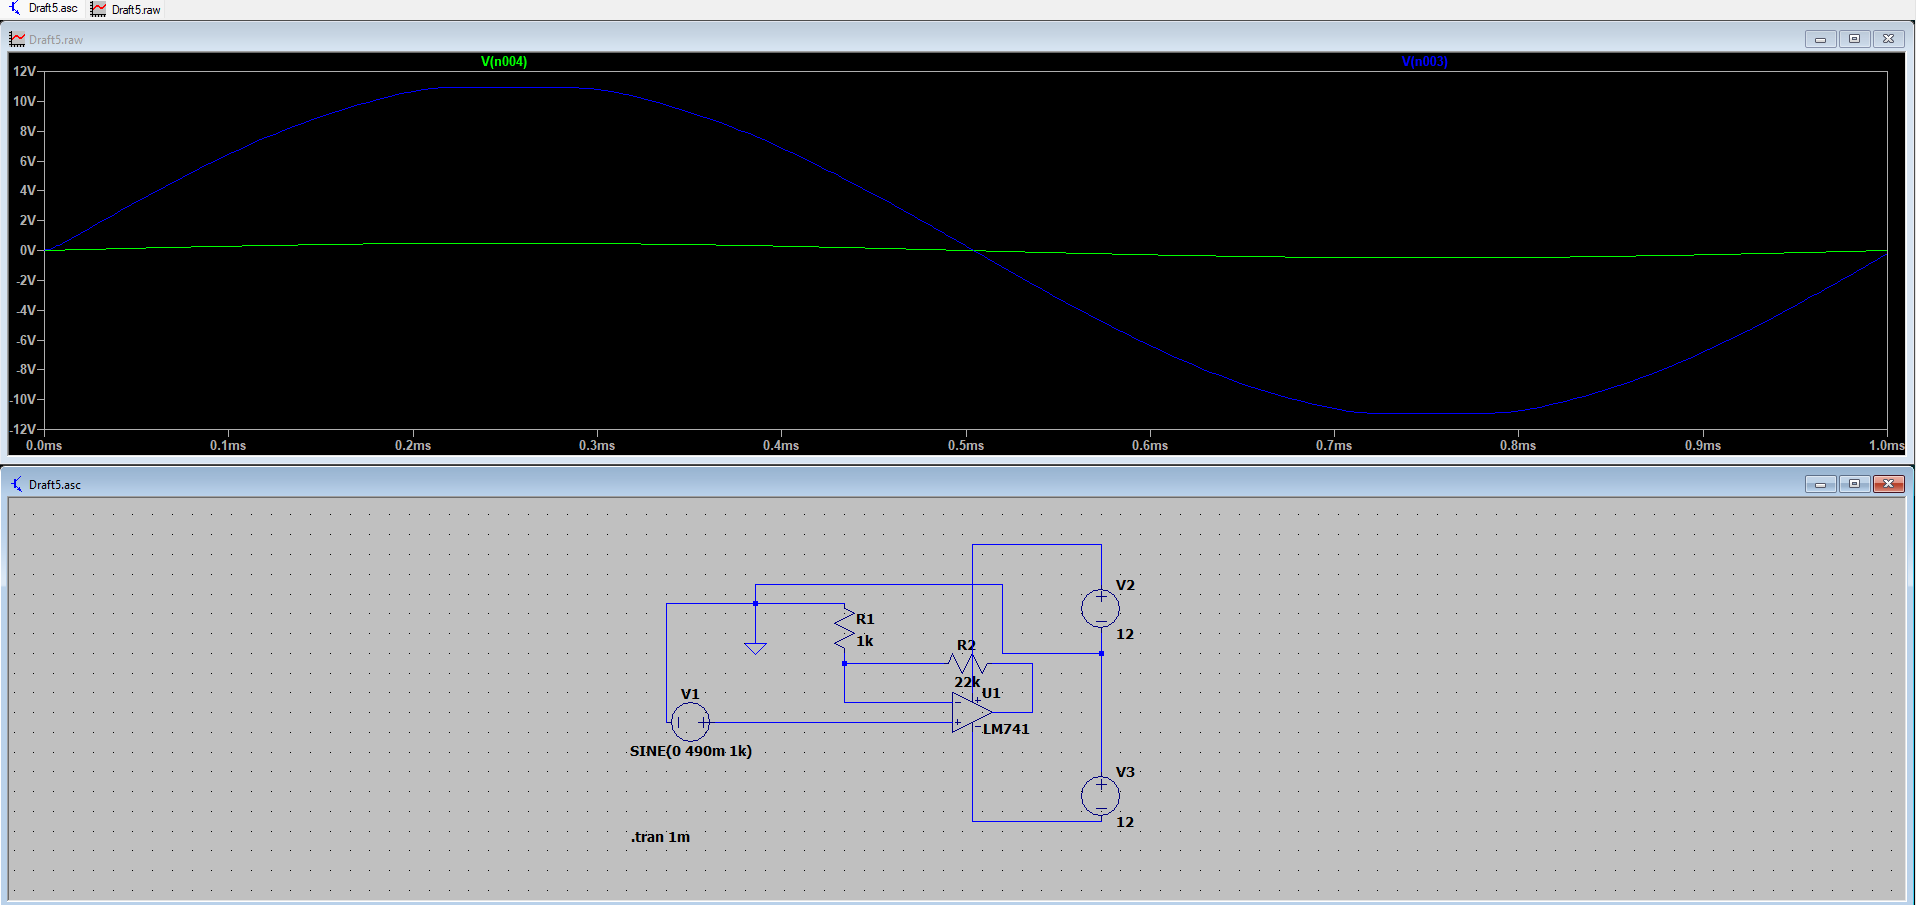
\includegraphics[width=1\textwidth]{assets/490m-non-inverting.png}
    \caption{Non-Inverting Amplifier @ 490mV}
    \label{fig:490m-non-inverting}
\end{figure}

Applying 490mV input to the non-inverting amplifier, the output should be 13.7V but it is limited to 12V due to the power supply as seen in Figure \ref{fig:490m-non-inverting}.

\newpage
\thispagestyle{plain}

\begin{figure}[h]
    \centering
    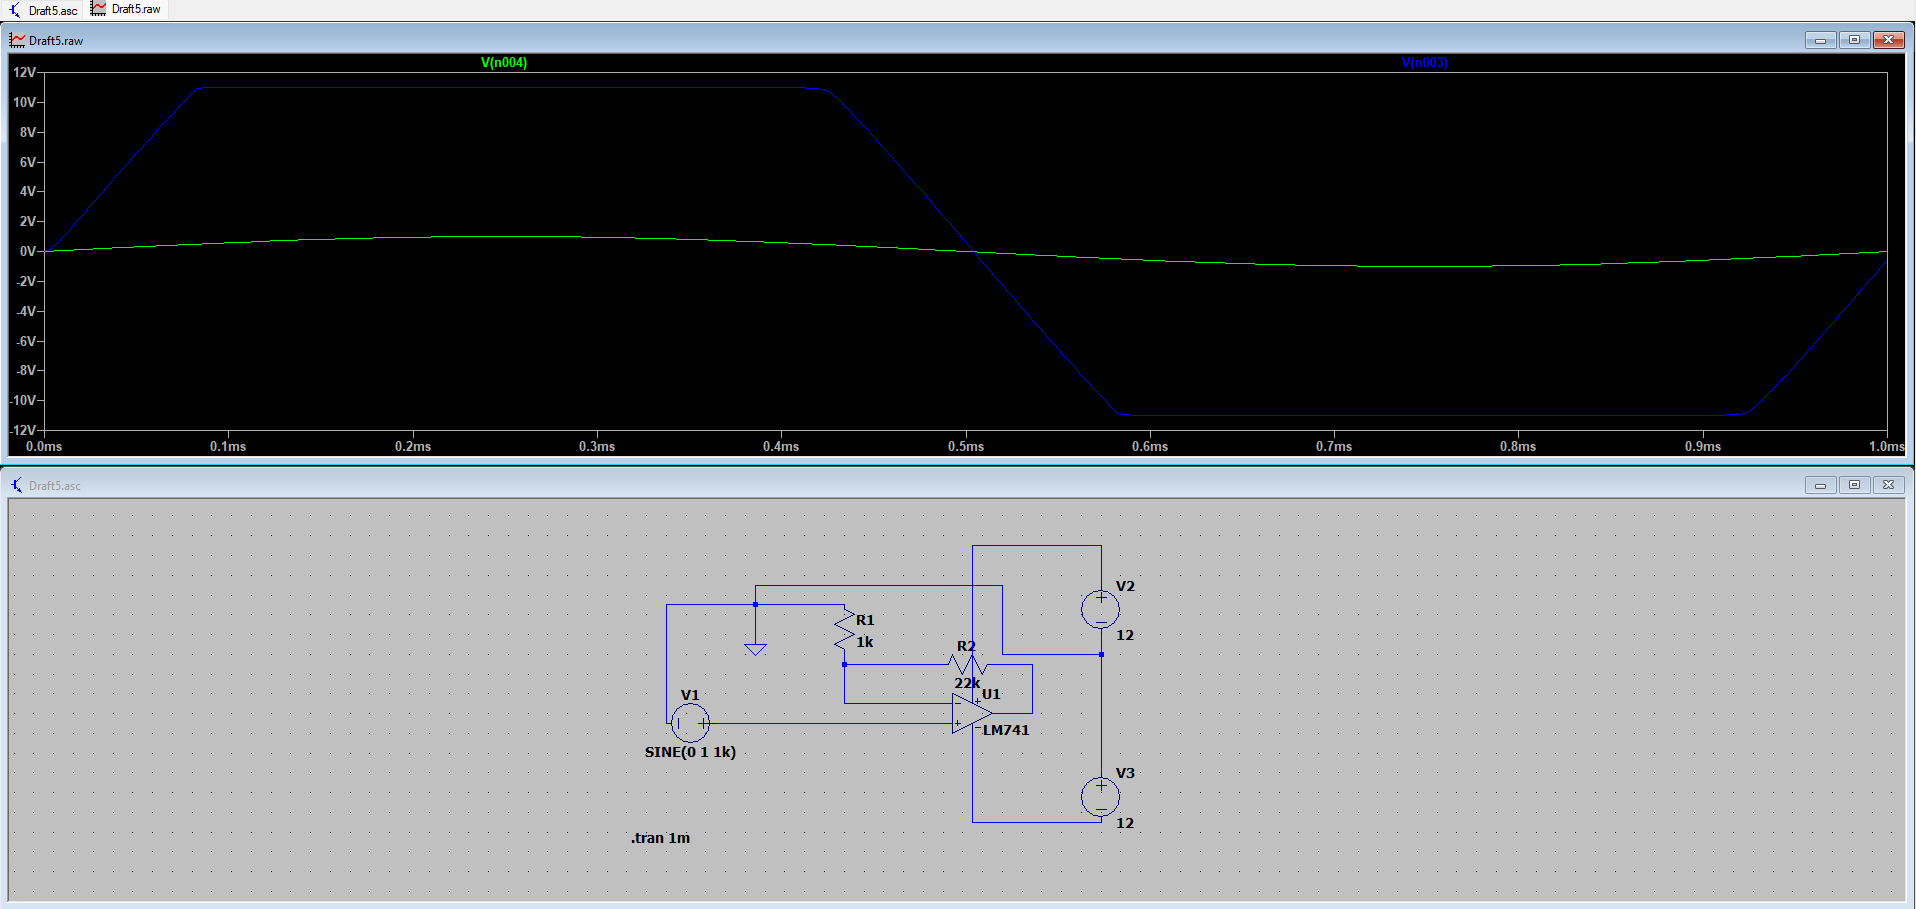
\includegraphics[width=1\textwidth]{assets/1-non-inverting.png}
    \caption{Non-Inverting Amplifier @ 1V}
    \label{fig:1-non-inverting}
\end{figure}

Applying 1V input to the non-inverting amplifier, the output should be 23V but it is limited to 12V due to the power supply as it is \textbf{more visible} in Figure \ref{fig:1-non-inverting}.

\newpage
\thispagestyle{plain}

\subsection{Inverting Amplifier}

\begin{figure}[h]
    \centering
    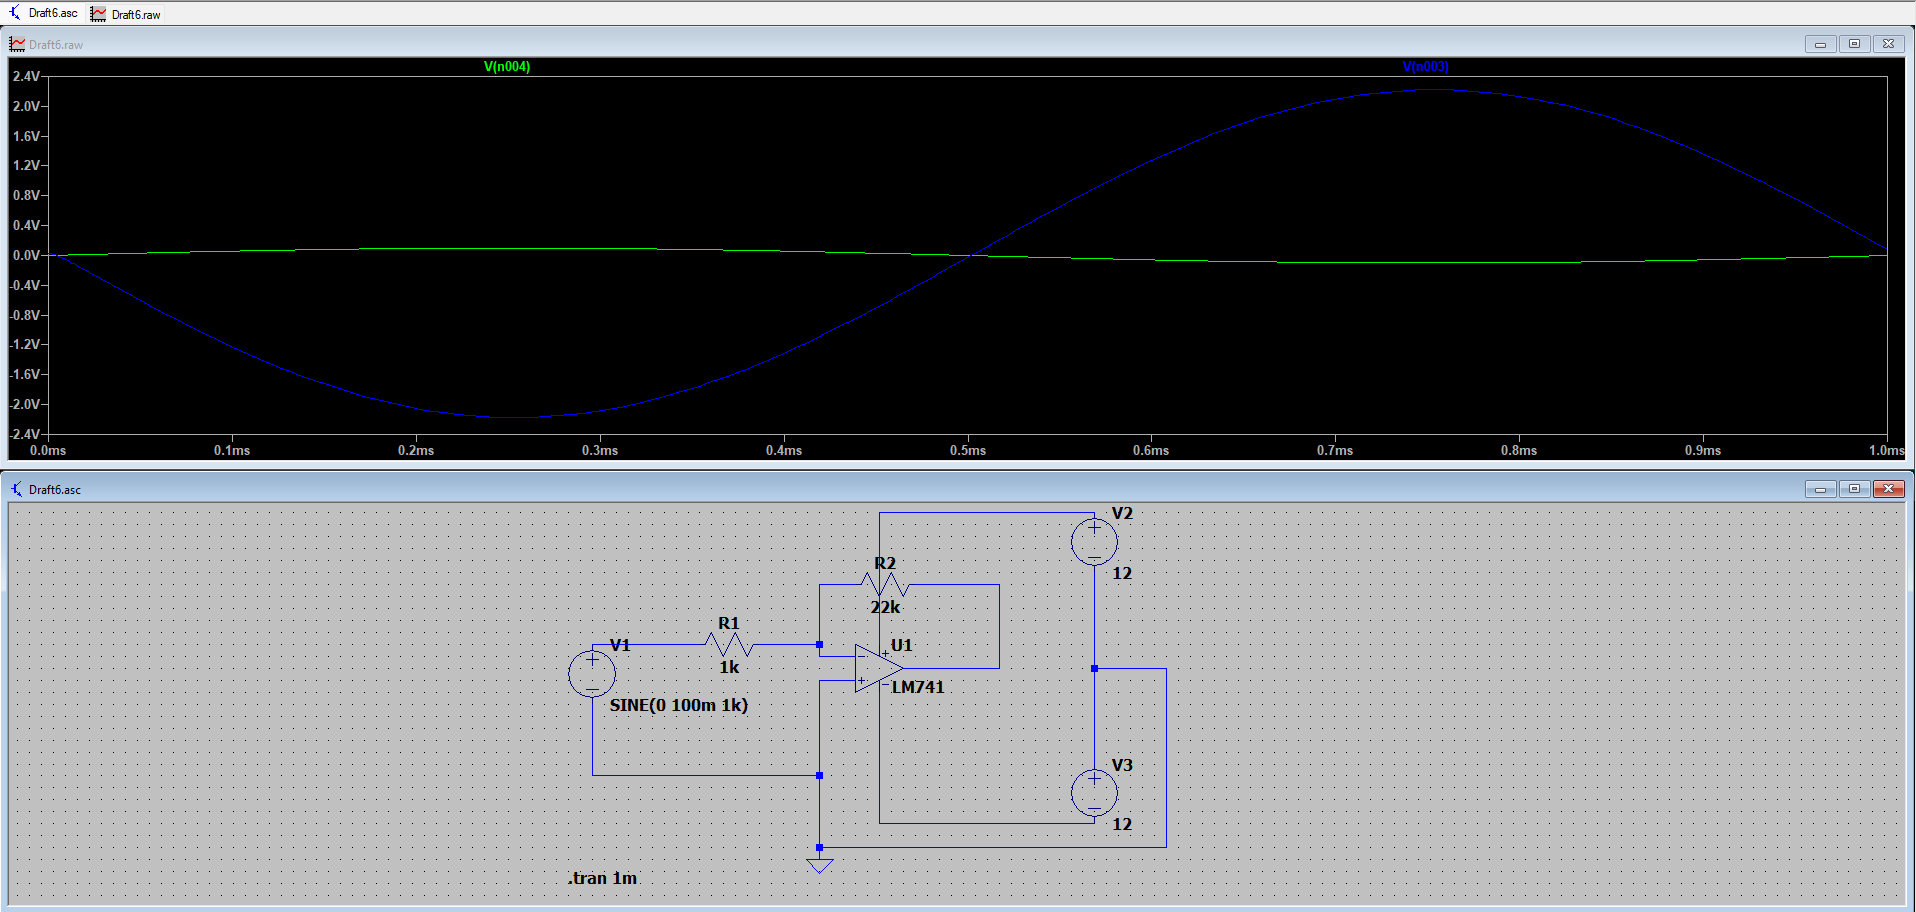
\includegraphics[width=1\textwidth]{assets/100m-inverting.png}
    \caption{Inverting Amplifier @ 100mV}
    \label{fig:100m-inverting}
\end{figure}

Applying 100mV input to the inverting amplifier, the output is -2.2V as expected. The simulation result is shown in Figure \ref{fig:100m-inverting}.

\begin{figure}[h]
    \centering
    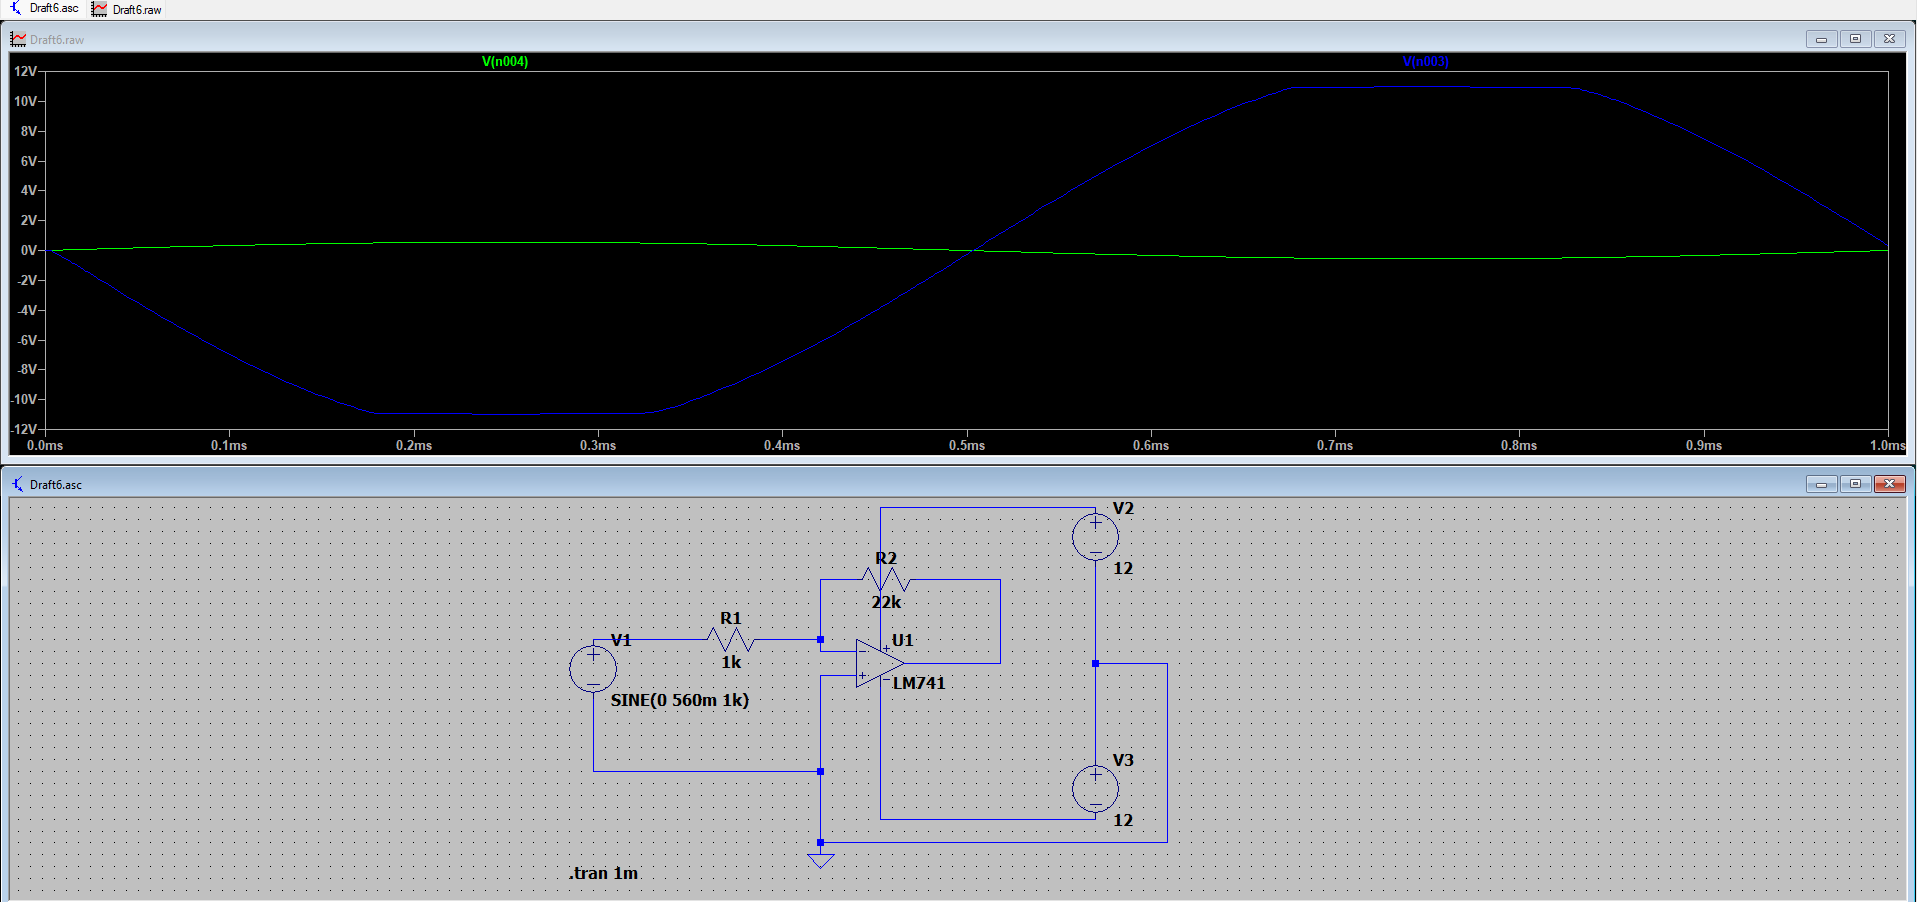
\includegraphics[width=1\textwidth]{assets/560m-inverting.png}
    \caption{Inverting Amplifier @ 560mV}
    \label{fig:560m-inverting}
\end{figure}

Applying 560mV input to the inverting amplifier, the output should be -12.32V but it is limited to -12V due to the power supply as seen in Figure \ref{fig:560m-inverting}.

\newpage
\thispagestyle{plain}

\begin{figure}[h]
    \centering
    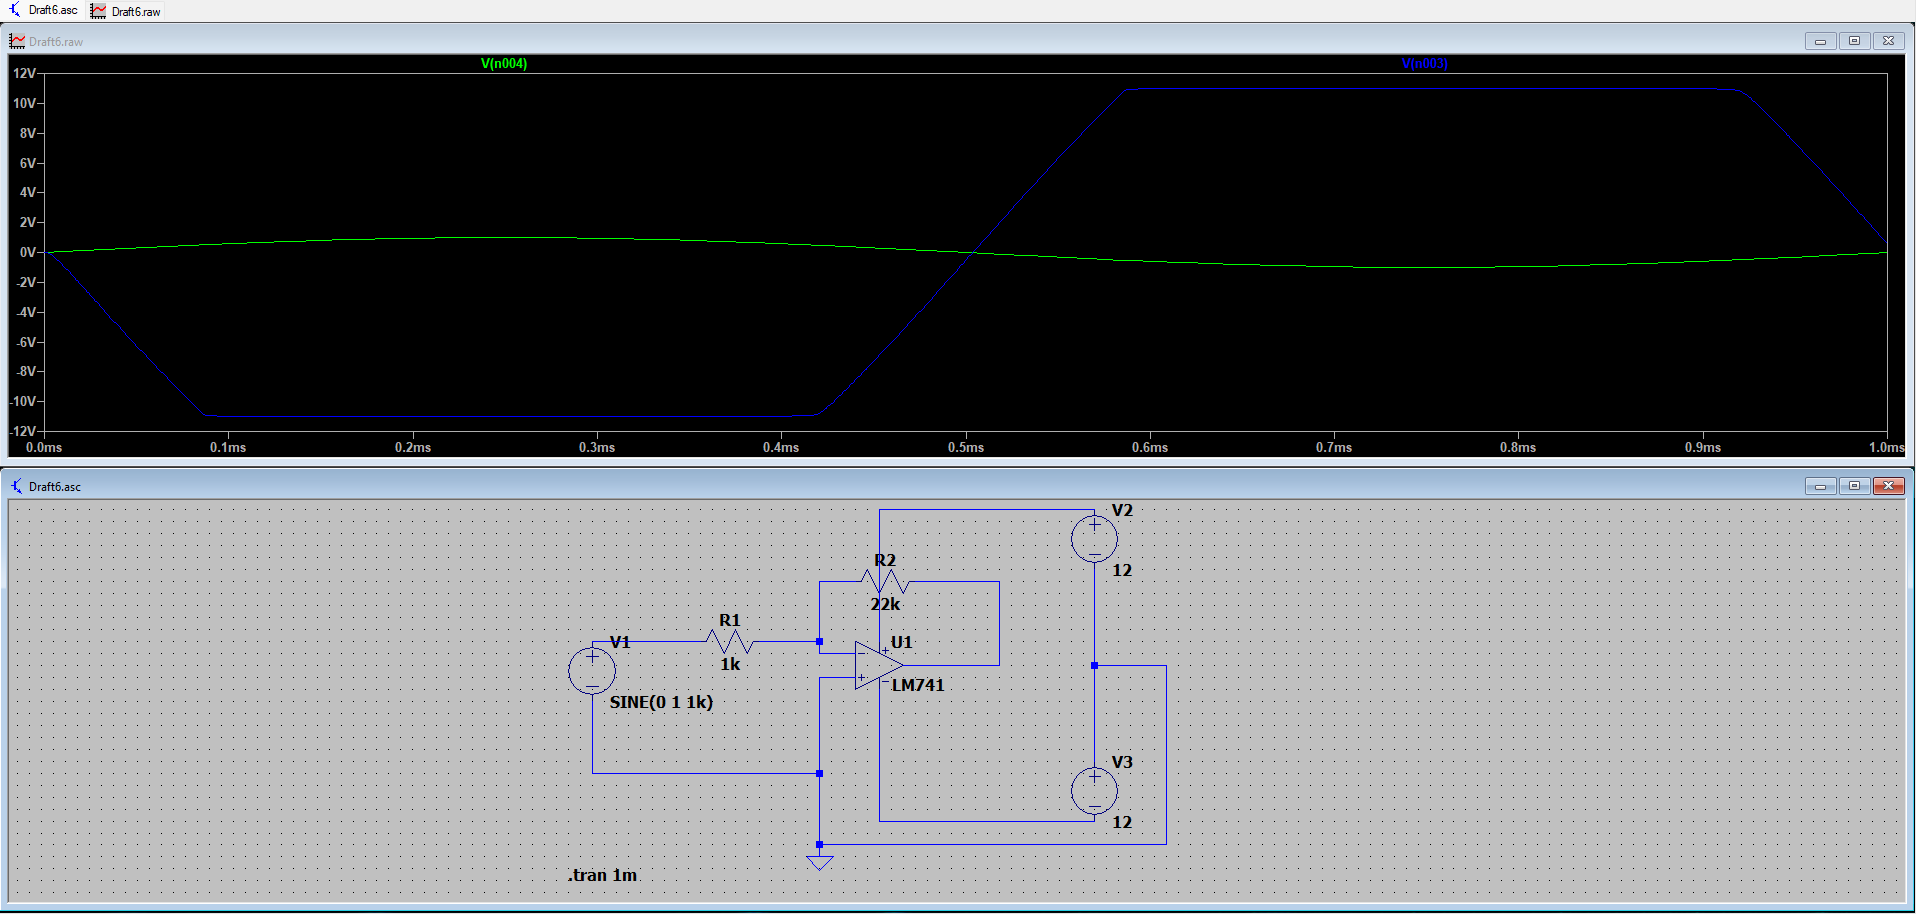
\includegraphics[width=1\textwidth]{assets/1-inverting.png}
    \caption{Inverting Amplifier @ 1V}
    \label{fig:1-inverting}
\end{figure}

Applying 1V input to the inverting amplifier, the output should be -22V but it is limited to -12V due to the power supply as it is \textbf{more visible} in Figure \ref{fig:1-inverting}.

